\documentclass{neu_handout}
\usepackage{url}
\usepackage{amssymb}
\usepackage{amsmath}
\usepackage{marvosym}
\usepackage{hyperref}
\usepackage{enumitem}
\usepackage{amsmath}

%\usepackage[demo]{graphicx}

\usepackage{graphicx}
\usepackage{subcaption}
\usepackage{caption}

%\usepackage{floatrow}
\usepackage{comment}
\pagenumbering{gobble}
\usepackage{hyperref}



\everymath{\displaystyle}

% Professor/Course information
\title{Packet: Pattern Recognition in Accidents in London}
\author{Adwait Sahasrabhojanee, Sreejith Sreekumar, Xue Yu, Xuexian Li}
\date{\today}
\course{DS 5230}{Unsupervised Machine Learning}

\begin{document}

\section{Introduction}
The UK government has put their efforts into building an aggregated collection of accident records in the England, Scotland and Wales regions
over a span of ten years from 2005 to 2014. The data includes 1.6 million accident instances. Having access to this, one of the most comprehensive data sets on traffic, we work towards
uncovering patterns and answer questions related to the potential causes and trends of accidents. We start our analysis on the whole of the UK area and eventually shift our emphasis towards
isolating and understanding urban cites where most accidents are concentrated, taking London as the candidate for our study.

\subsection{The Dataset}
We consider the accident data from years 2009 to 2014 for our experiments. Every record of an accident includes the location (in geographical co-ordinates), the type of area, and the date and time of the accident. In addition, it includes the speed of the vehicle, the severity, the number of officers attended, the number of casualties, the weather conditions, the road and lighting conditions during the accident. \\

Furthermore, to understand the flow of traffic, we are given the Annual Average Daily Flow data that tracks the amount of traffic which are present on the roads in the UK, at different points of time. \\

\section{Exploring our data}
We begin our analysis, identifying the areas where accident concentrations are the highest. The towns/cities where the accident occurred were identified by decoding the geo-tags, and the top 200 places where the concentration is the highest were isolated. The records from these 200 places were tagged on a map to see the spread of hotspots. As we can see from the map, these hotspots are centered around the main cities in the UK.

\begin{figure}[!htb]
\minipage{0.5\textwidth}
  \includegraphics[width=\linewidth]{map1.png}
  \endminipage\hfill
\minipage{0.5\textwidth}
  \includegraphics[width=\linewidth]{map2.png}
\endminipage
\end{figure}

These regions, which we have identified to be the hotspots are also the highest populated cities[1], as well as the most traffic dense regions in the UK(Appendix, Fig 1). \\

Looking into the summary statistics of the data, we realized that most accidents occur leaving at least one casualty. Most accidents involve two vehicles, or a pedestrian and a vehicle. It is also noteworthy that the accidents are neither decreasing nor increasing consistently during the years under consideration. The numbers of accidents in a year stays around 150000, with  an increase of over 175000 in 2012 (Figure 1). We could also see that the number of accidents peak during the hours from 5.00pm to 6.00pm and between 8.00am to 9.00 am (Figure 2). These are typically the hours when people commute to their workplace and back home. This could be an early indicator that the increase in traffic could be a significant cause of the number of accidents, or rather the roads are not well equipped to contain it. \\

\begin{figure}[!htb]
\minipage{0.32\textwidth}
  \includegraphics[height=3.80cm, width=.9\linewidth]{counts.png}
  \caption{Frequency of Accidents}\label{fig:frequency}
\endminipage\hfill
\minipage{0.32\textwidth}
  \includegraphics[width=\linewidth]{hour-study.png}
  \caption{Hourly variations}\label{fig:hour-study}
\endminipage\hfill
\minipage{0.32\textwidth}
  \includegraphics[height=3.75cm, width=\linewidth]{day-study.png}
  \caption{Daily trends}\label{fig:day_study}
\endminipage
\end{figure}

Considering that there are UK has four distinct seasons with significant variations in climate, we were inclined to check the possibility of skew in the distribution of accidents across seasons
and light conditions. \\

\begin{figure}[!htb]
\minipage{0.5\textwidth}
  \includegraphics[width=\linewidth]{weather-study.png}
\endminipage\hfill
\minipage{0.5\textwidth}
  \includegraphics[width=\linewidth]{lighting-study.png}
  \endminipage
\caption{Trends in accidents - Weather and Lightning conditions}  
\end{figure}

From the plots(Figure 4), we conclude that the number of accidents that happen during perfectly good weather are much higher in count compared to the climatic conditions which could possibly affect the normal traveling conditions adversely. In addition, it is seen that the count of accidents in daylight are far more than the rest. This analysis makes it evident that neither of these two is the root cause of accidents. \\

Moving forward from this point, we narrowed our focus to metropolitan cities in the United Kingdom. This is because for every clustering or unsupervised algorithm that we used to analyze the data, the results converged into two regions - Urban or Rural. We realized that this is because of the large differences in attribute values in urban and rural areas (Appendix:Figure 10). Since London consistently  tops in the frequency of accidents and in search of more interesting results, we chose it to be the candidate region for our analysis.

\section{Data Mining Analysis}

\subsection{Investigation of Patterns in Traffic - London}
Streets in the UK are uniquely identified by an alpha-numeric numbering scheme[6]. Concatenating this identifier with the Northing and Easting co-ordinates makes a good marker for us to uniquely identify an accident spot or a street fragment without losing information about the street. The Annual Average Daily Flow (AADF) of traffic was analyzed to cluster the traffic dense regions in London. \\

Road fragments with similar characteristics in traffic were identified though cluster analysis. \textit{K-means} was our candidate algorithm. Variables that quantify traffic of a region were manually selected, which included number of motor cycles, number of taxis, and the number bus coaches. The  experiment was performed with same parameters for every year between 2009 and 2014 to study the variations in areas with high traffic density. \textit{Silhouette method} was used to determine the optimal number of clusters, which was discovered to be two (Appendix:Figure 11).\\

Examining the clusters, we could see that the density of traffic in spots belonging to one of the clusters is very high compared to the ones in the second cluster. The co-ordinates of points belonging to this cluster was dropped on a map and it turns out that they are very close to each other - They collectively represent larger road fragments where the traffic is the highest. We plotted yearly heatmaps of accidents to study how they correlate with the traffic flow plots. It can be observed that there is a positive correlation between the hotspots where traffic density is the highest, and the number of accidents. In other words, the high traffic flow zones in London are also accident prone areas. To illustrate this at one of the locations, consider the map segment which shows the traffic flow density on street A41 between Edgware Road(Circle District and Hammersmith \& City) and Baker Street[Figure 5: Left]. The right end of figure 5 shows the heatmap of accidents in the same fragment. This is a good indication that the traffic dense fragments are not equipped enough to contain the traffic. \\

\begin{figure}[!htb]
\minipage{0.5\textwidth}
  \includegraphics[height=6cm, width=\linewidth]{traffic-bakers-street.png}
\endminipage\hfill
\minipage{0.5\textwidth}
  \includegraphics[height=6cm, width=\linewidth]{accident-2009-heatmap-bakers-street.png}
  \endminipage
\caption{Traffic density and accident spot correlation - Marylebone Road, London}  
\end{figure}



\subsection{Segregation of Accidents in London using numeric attributes}

Our dataset has seven variables that are either ordinal or binary. Using \textit{k-means} and \textit{DBSCAN} we performed clustering on these variables, segregate accidents and interpret the clusters. Our motivation for doing this was to look at a large cluster, and figure out the causes of the accidents in the largest cluster and suggest a solution to reduce the accidents in the entire cluster. \\

Prior to DBSCAN, we applied \textit{Principal Component Analysis} to reduce the time it takes to converge.   The first six components explained about 95\% of the variance. We thus managed to lower the number of dimensions by 1(Figure 6). \\

\begin{figure}[!htb]
    \begin{center}
      \includegraphics[height=6cm,keepaspectratio]{pca.png}
      \caption{Cumulative Proportion of Variance Explained by Principal Components}
    \end{center}
 \end{figure}

We experimented with a variety of parameter combinations for the cluster analysis. For a lot of combinations, DBSCAN clustered the data into two clusters, depending on whether they are from Downtown London, or the surrounding boroughs [Figure 7]. Upon further exploration, we discovered that one of the variables - Police Force, was very high for accidents in Downtown London, and very low everywhere else. \\

\begin{figure}[!htb]
    \begin{center}
      \includegraphics[height=5cm, keepaspectratio]{db_1_county.png}
      \caption{DBSCAN Clustering on numeric columns separates one borough from the others (Cluster 0 indicates outliers)}
    \end{center}
\end{figure}

We removed the \textit{Police Force} variable, and repeated the clustering experiments. Unfortunately, the results were not fruitful. This could be because of the fact that although the number of records are quite high, there are not a large number of unique values that its numeric variables could take. For example, Accident Severity could only take a value of 1, 2 or 3. This prompted us to focus on some of the nominal variables instead. \\

\subsection{Road and Lighting Conditions}

We discovered that the majority of accidents happen either in the daylight or when the street lights are present and lit in the darkness [Figure 4]. Additionally, looking over the conditions of the surface of the roads during the accidents, we see that a very large number of accidents occur on dry roads. Also, we noticed that around 20\% of the total number of accidents every year in Greater London happen when the roads are wet and damp. However, Greater London receives most of its rain during the months of Oct - Jan[5], and there is a chance that 20\% of accidents occur when the roads are wet because roads are wet 20\% of the time. Exploring the surface conditions in Greater London during different months, we found that accidents on wet roads are present throughout the year.\\

We clustered the accidents based on Road Surface Conditions, Carriageway Hazards, Special Conditions at Site, and Light Conditions, which were all nominal variables. We used the \textit{Dice co-efficient} as a distance metric for these columns, and then clustered them using the \textit{k-medoids algorithm}. K-medoids work mostly the same way as k-means, with a couple of differences. Unlike k-means, k-medoids always selects data points as the centers, for every iteration. This makes it a viable option for nominal data, as clustering around a point that does not exist in the dataset only makes sense for continuous or ordinal variables. Also, k-medoids uses the Manhattan Distance, and not the Euclidean Distance, as is common in k-means [7]. The silhouette scores were computed for k = 2 to 10, and a k of 4 was chosen (Appendix: Figure 12), having a silhouette of 0.95. \\

\begin{figure}[!htb]
    \begin{center}
      \includegraphics[height=9cm, scale=0.01,keepaspectratio]{4_clusters.png}
      \caption{Clustering for Road and Lighting conditions}
    \end{center}
\end{figure}

Visualizing a few data points from each cluster, it can be seen that the Light Conditions and Road Surface Conditions variables have been given importance by the clustering algorithm, and the four clusters are four combinations of these two variables. The accidents belonging to each cluster plotted on maps are shown above(Figure 8). \\ 



The plots of the four clusters show that two of the clusters (red and orange) contain a much higher \textit{proportion} of accidents that occurred away from Downtown London than the other two clusters. \\


As can be seen in (Appendix:Figure 13), the common important variable between these clusters is the road surface condition. It would seem from this clustering that a Wet/Damp road has a higher chance of causing an accident as you move away the heart of the city. \\ 

A possible explanation for this could be the increase in speed limit as we head out of Downtown London (Appendix: Figure 14). People going faster on wet roads would have a much higher chance of losing control of their car as compared to people going slower on wet roads. \\

\section{Discussion}
Looking at the results of our analysis, we see that certain road fragments on the roads of London, are particularity traffic dense. These same spots are highly accident prone, indicating that these roads are not equipped to handle the amount of traffic that they get. We further observed that wet or damp roads have a higher chance of causing an accident as you move away the heart of the city, which can be explained by the higher speed limit at the outskirts of the city. The clusters show that the risk that comes with driving fast on wet/damp roads is much higher than the risk associated with driving fast on dry roads. \\

Based on our observations, we propose the following in the roads of London.  These suggestions will potentially be able to reduce the number of accidents that happen in the Greater London area:

\begin{itemize}
\item{Build stack interchanges near roads A127, A3220, A312, M11, A3, A102, A41, M4, M1, A40, A2, A316, A1203, M25, A406, A1261, A4202, A13, A12, A4, A501, A3211, A20. The traffic redirected by stack interchanges will reduce the traffic density in this accident-prone area.}

\item{Reduce the speed limit in the boroughs on the outskirts of Greater London during the months in which rain is most likely to fall. Implementing this change will not require any money, except for the money that will be spent on road signs.}

\end{itemize}

\section{Project Details}
\begin{itemize}
\item Analysis Code : \url{https://github.com/srjit/kaggle-uk-accident-data-analysis/} \\
  Instructions for running code have been put in the \textbf{README} files of the respective folders.
\item Youtube link of the presentation : \url{https://www.youtube.com/watch?v=mATNx7Pn1ro}  
\end{itemize}

\pagebreak

\section{References}
 [1] \url{http://www.citymayors.com/gratis/uk_topcities.html}
\newline
 [2] \href{https://data.london.gov.uk/dataset/statistical-gis-boundary-files-london}{London Shapefile}
 \newline
 [3] \href{http://www.naturalearthdata.com} {UK Shapefile}
 \newline
 [4] \href{https://en.wikipedia.org/wiki/Demography_of_the_United_Kingdom}{Demography of the United Kingdom}
 \newline
 [5] \href{http://projectbritain.com/climate.html}{London Yearly Rainfall Distribution}
 \newline
 [6] \href{https://en.wikipedia.org/wiki/Great_Britain_road_numbering_scheme}{Great Britain road numbering scheme}
 \newline
 [7] \href{https://en.wikipedia.org/wiki/K-medoids}{k-medoids}
 \newline
 [8] Chavent M, Kuentz Simonet V, Liquet B, Saracco J (2012) ClustOfVar: An R Package for the Clustering of Variables. Journal of Statistical Software 50(13)

 
\section{Appendix}
\begin{figure}[!htb]
  \includegraphics[width=8cm, height=10cm]{vehicles-by-county.png}
  \caption{Frequency of vehicles per county}
\end{figure}


\begin{figure}[!htb]
\minipage{0.5\textwidth}
  \includegraphics[height=10cm,width=0.8\linewidth]{accident-severity.png}
\endminipage\hfill
\minipage{0.5\textwidth}
  \includegraphics[height=10cm,width=0.8\linewidth]{population-density.png}
  \endminipage
\caption{Accident Severity and Population Density in different regions in the UK}  
\end{figure}

\begin{figure}[!htb]
    \begin{center}
      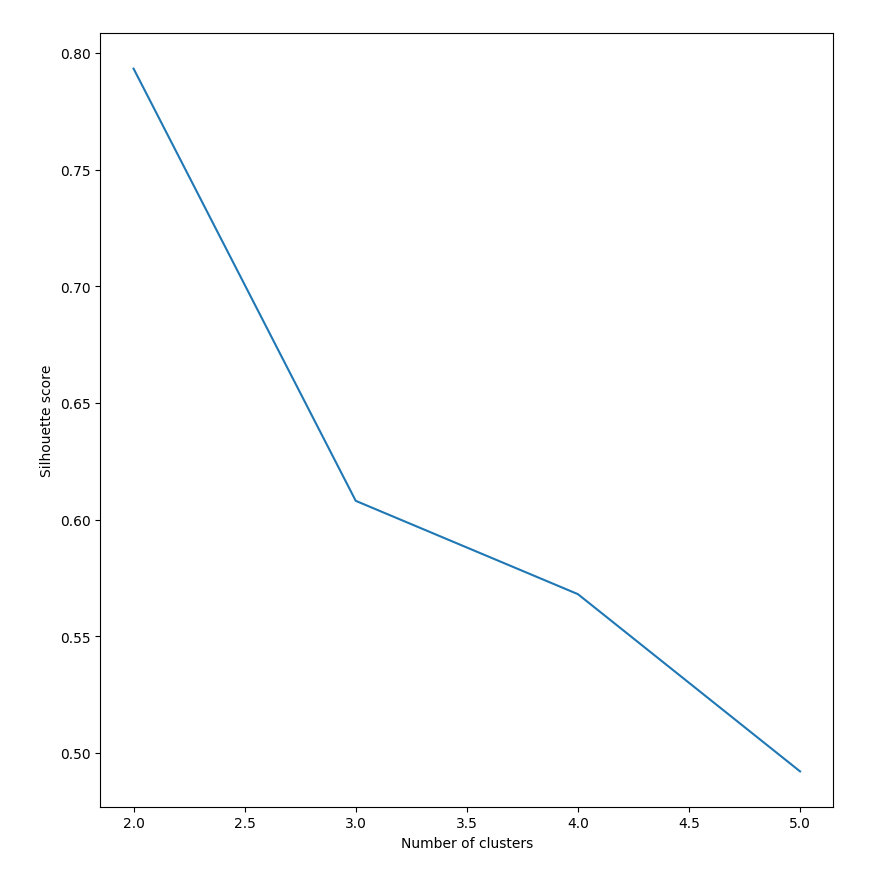
\includegraphics[height=7cm]{silhouette-score-traffic.png}
      \caption{Silhouette score for Traffic Clustering}
    \end{center}
\end{figure}

\begin{figure}[!htb]
    \begin{center}
      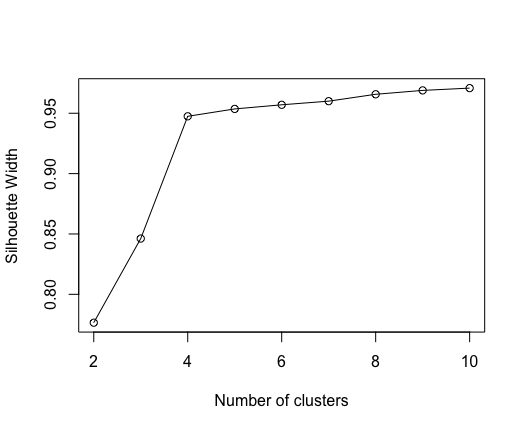
\includegraphics[height=5cm]{silhouette_road_conditions.png}
      \caption{Silhouette score for Road Conditions Clustering}
    \end{center}
\end{figure}


\begin{figure}[!htb]
    \begin{center}
      \includegraphics[height=2.75cm,width=17cm]{cluster-eg.png}
      \caption{Examples of Clustered Datapoints for Road and Lighting conditions}
    \end{center}
\end{figure}


\begin{figure}[!htb]
    \begin{center}
      \includegraphics[height=7cm,keepaspectratio]{sl_london.png}
      \caption{Accidents by Speed Limit (Excluding the Ubiquitous Speed Limit of 30)}
    \end{center}
\end{figure}

\begin{figure}[!htb]
    \begin{center}
      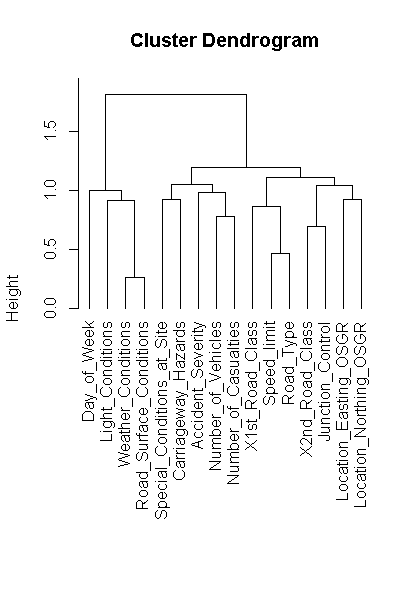
\includegraphics[height=7.5cm,keepaspectratio]{Dendrogram-of-variable-cluster.png}
      \caption{Cluster Dentogram from Hierarchical Clustering of Variables}
    \end{center}
\end{figure}


\end{document}

%%% Local Variables:
%%% mode: latex
%%% TeX-master: t
%%% End:
